\begin{frame}{Qualitative results: Our system}
  % Show some impressive qualitative results that are better than naive
  % initialization
  \centering
  \includemedia[label=allenergies,
    width=\linewidth,height=0.6\linewidth, % 16:9
    activate=pageopen,
    addresource=graphics/allenergies.mp4,
    flashvars={
      source=graphics/allenergies.mp4
      &loop=true             % loop video
      &scaleMode=letterbox   % preserve aspect ratio while scaling the video
    }
  ]{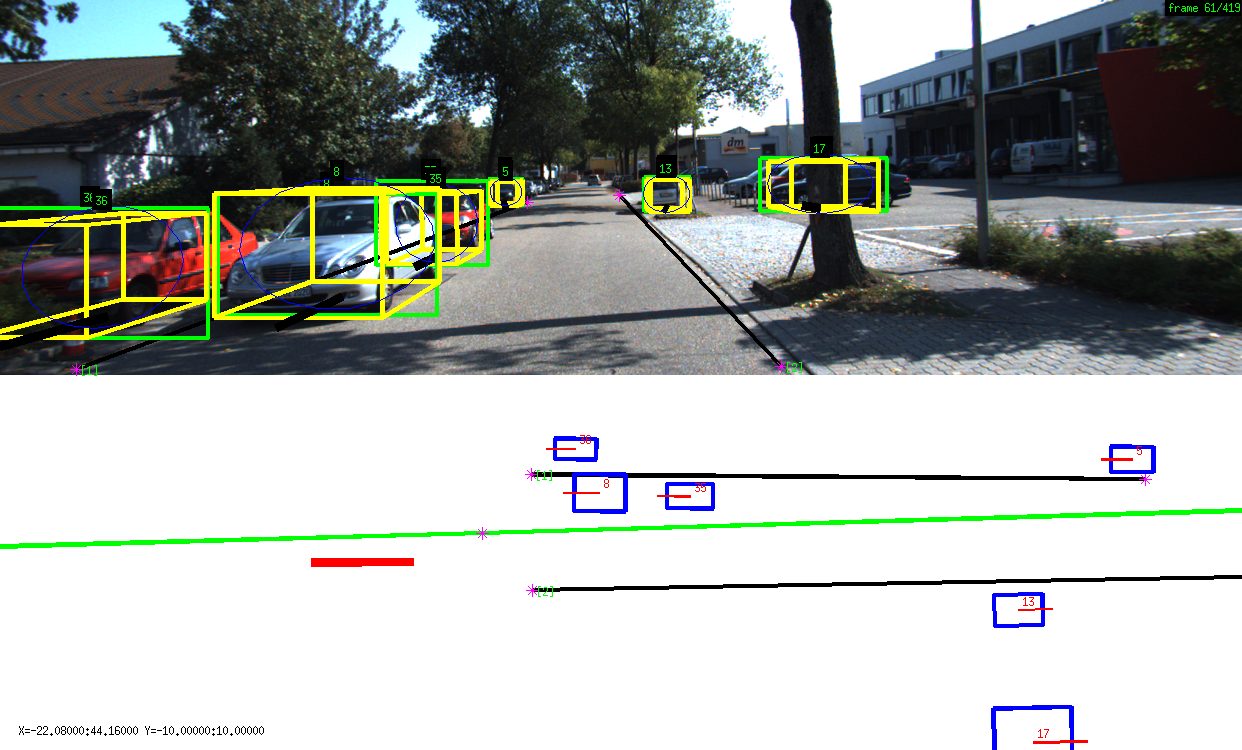
\includegraphics{graphics/0000000061_bevdown.png}}{VPlayer.swf}
\end{frame}

\begin{frame}{Quantitative results}
  % Show that quantiative results are still negative but ...
  \small{
    t : Mean translation error in ground plane per traffic particpant per frame

    yaw : Mean yaw error in ground plane per traffic particpant per frame

    dim : Mean dimension error in ground plane per traffic particpant per frame

\begin{table}
  \begin{tabular}{lrrr}
    \toprule
    Energy & t & yaw & dim \\
    \midrule
    initialization                                                                                  & 3.79 & \textbf{0.86} & 1.64 \\
    $\EnergyLane+\EnergySize+\EnergyBBox+\EnergyDyn                                       $ & 3.83 & 0.90 & \textbf{1.14} \\
    %$\EnergyLane+\EnergySize+\EnergyBBoxocc+\EnergyDyn                                    $ & 3.83 & 0.90 & 1.14 \\
    %$\EnergyLane+\EnergySize+\EnergyBBoxocc+\EnergyDyn+\EnergyCol                         $ & 3.92 & 0.91 & 1.15 \\
    %$\EnergyLane+\EnergyContpttracks+\EnergySize+\EnergyBBoxocc+\EnergyDyn             $ & 3.81 & 0.92 & 1.59 \\
    $\EnergyLane+\EnergyTrackNoOcc+\EnergySize+\EnergyBBox+\EnergyDyn+\EnergyCol $ & 3.80 & 0.91 & 1.58 \\
    $\EnergyLane+\EnergyTrack+\EnergySize+\EnergyBBox+\EnergyDyn+\EnergyCol   $ & \textbf{3.78} & 0.91 & 1.58 \\
    \bottomrule
  \end{tabular}
\end{table}
  }

\end{frame}

\begin{frame}{What is wrong with the results?}
  % Outliers in point tracks
  % Outliers in detections
  % Poor inference methods
  \begin{itemize}
    \item Inference is slow
    \item Learning parameters is difficult with slow inference
    \item Poor parameters cause poor results
  \end{itemize}
  % Parameter learning
  % Simplify graphical model
  % Approximate graphical model to a tree
  % Use discretization for belief propagation followed by gradient descent
\end{frame}
\begin{frame}{What to do?}
  \begin{itemize}
    \item Speedup inference
    \item Simplify graph by \cite{chow1968approximating} tree approximation
    \item Use belief propagation for faster inference on trees
  \end{itemize}
  
\end{frame}

\begin{frame}{Conclusion}
    Our occlusion aware 3D modeling improves association\\
    ... but requires more work to show improvement on localization
\end{frame}
